\section{Discussion and Analysis}

\subsection{Which Base Model is the best for LoRA Fine-tuning?}

Mistral-7B and Zephyr-7b-beta emerge as leaders, albeit in different categories. Mistral-7B frequently achieves top performance across the most number of tasks (10/31), suggesting a high adaptability (Figure \ref{fig:topperformer}). Conversely, Zephyr boasts the highest overall average performance (0.731). Mistral-7b, Mistral-7b-instruct, and Zephyr-7b-beta (which is itself based on Mistral-7b-instruct~\cite{66zephyr}) lead the pack for LoRA fine-tuning performance, ahead of Llama, Phi, and Gemma families.

\begin{figure}[ht]
    \centering
    \scalebox{0.7}{
    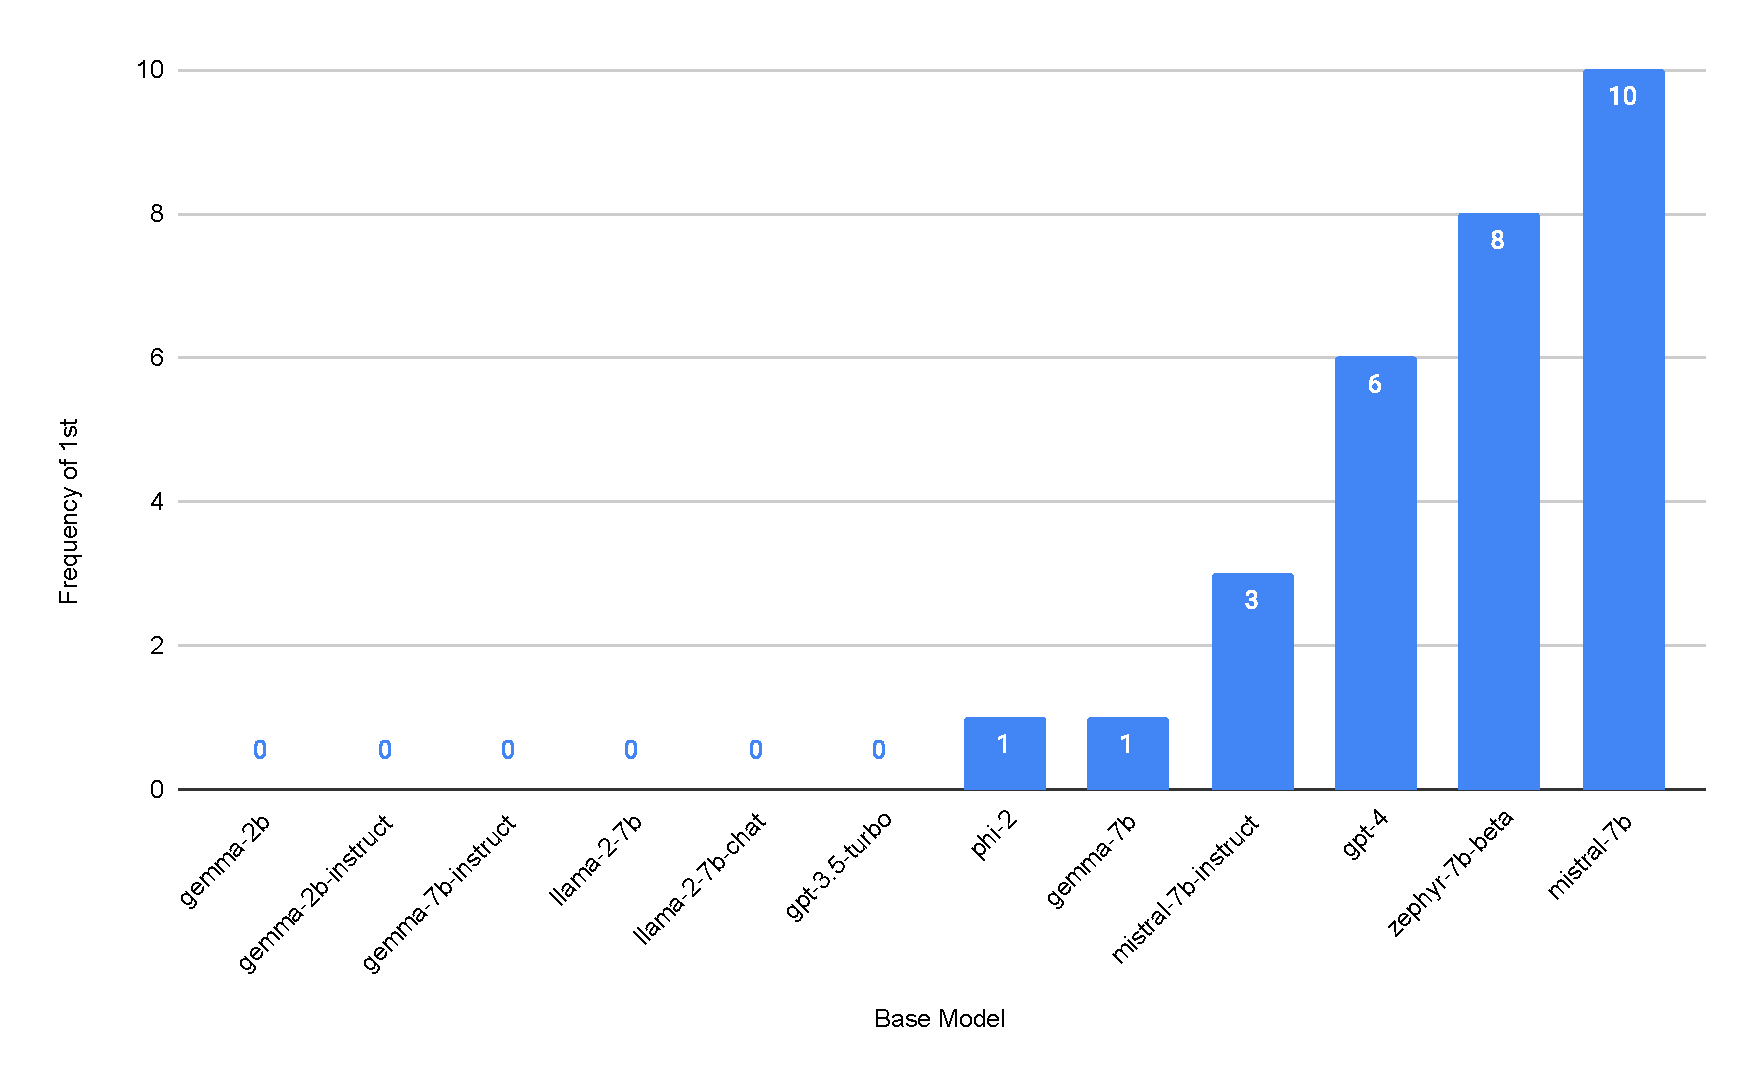
\includegraphics[width=\textwidth]{figures/top_performer.pdf}
    }
    \caption{Frequency of base models (with fine-tuning) as the top performer for a task. Ties, namely for the \textit{customer\_support} task where most models attain 100\% perfect scores, are excluded.}
    \label{fig:topperformer}
\end{figure}


\subsection{Does size matter for LoRA fine-tuning? 2B vs. 7B}

The 2B parameter Phi-2 model, after fine-tuning, outperforms all of the 2B and 7B Gemma models by overall overage, and is only 1.9 points behind the next highest performing 7B model, Llama-2-7b (0.677 vs. 0.696). Despite this, we find that fine-tuned 7B models are almost always better than fine-tuned 2B models (29/31 tasks). Among 2B parameter models in particular (Phi and Gemma), we see that all Gemma instruct models were better than Phi out of the box, however, Phi-2 performs better than all other Gemma models after fine-tuning.

\subsection{Is fine-tuning better with Instruction-tuned or Auto-complete models?}

In Figure \ref{fig:autocompletevsinstructiontuned}, we observe that before fine-tuning, instruction-tuned models outperform auto-complete models, despite using completion style prompts. A qualitative analysis shows that auto-complete models were much more likely to "go off the rails", and generate long irrelevant text sequences, and instruction-tuned models demonstrate a higher consistency in correctly attempting the imminent task.

After fine-tuning, the performance disparities between the models narrow. The average instruction-tuned model slightly outperforms the average auto-complete model by a margin of +0.009, however the reverse is true when comparing the best fine-tuned instruction-tuned model and the best fine-tuned auto-complete model (-0.002). Auto-complete models, possibly due to their broader and less specialized knowledge base, may be inherently more adaptable to a variety of tasks. However, with adequate fine-tuning, both types of models achieve comparable performance levels. We encourage further research to explore how the foundational design of instruction-tuned models influences their adaptability and effectiveness in task-specific fine-tuning.

\begin{figure}[ht]
    \centering
    \scalebox{0.7}{
    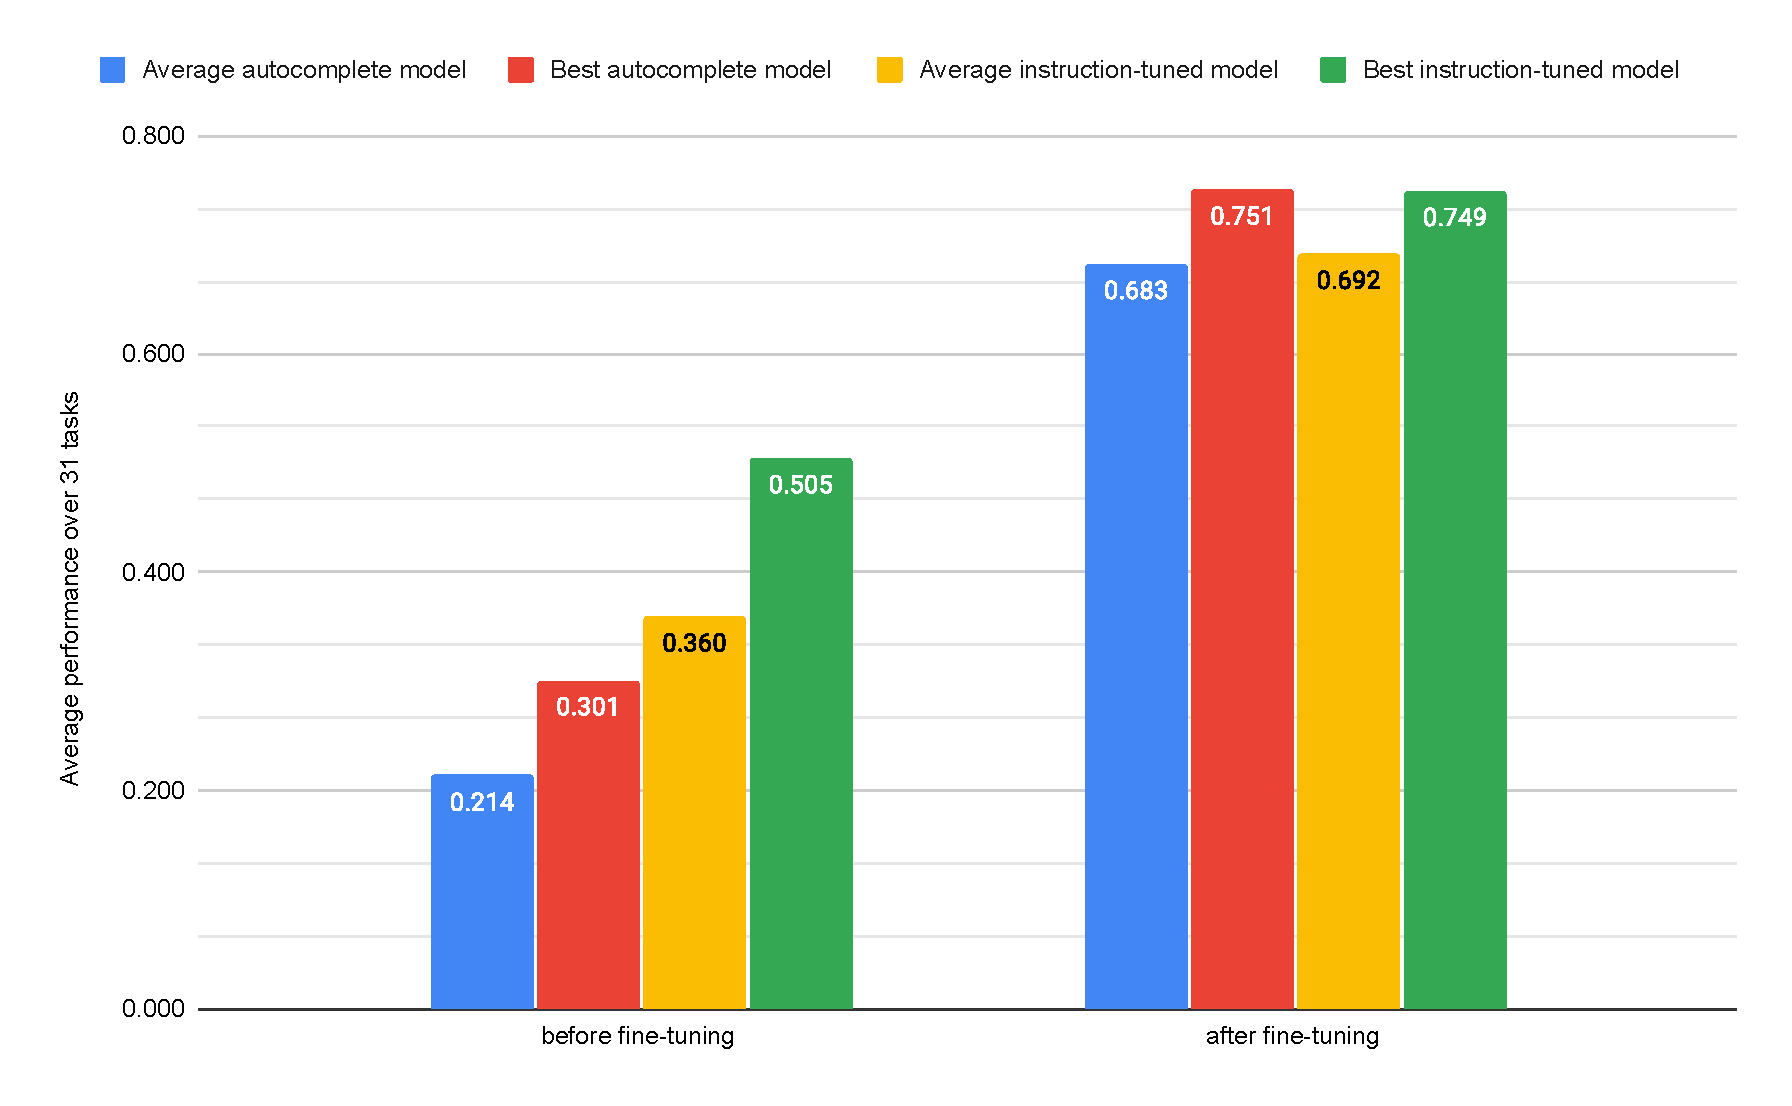
\includegraphics[width=\textwidth]{figures/autocomplete_vs_instruction.pdf}
    }
    \caption{Comparison of auto-complete vs. instruction-tuned base models, before and after fine-tuning.}
    \label{fig:autocompletevsinstructiontuned}
\end{figure}

\subsection{When does GPT-4 consistently outperform fine-tuned models?}

We observe a distinct advantage for fine-tuned LLMs on narrowly-scoped tasks, such as those within the GLUE benchmarks. These tasks, primarily classification-oriented, saw fine-tuned LLMs achieve near 90\% accuracy, outperforming GPT-4. GPT-4 continues to outperform fine-tuned models in 6 out of 31 tasks, particularly in broader, more complex domains such as Python coding and MMLU.

\subsection{Quantifying the relationship between fine-tuning quality lift and task complexity}

If fine-tuned models perform better on specialized "narrow" tasks and worse on "broader" tasks,  can we establish a predictive relationship between the complexity of a task and the efficacy of LoRA fine-tuning?  Identifying such a relationship could provide a valuable predictive tool for assessing the potential benefits of fine-tuning enhancements on new tasks before the fine-tuning process begins.

\subsubsection{Heuristics for fine-tuning quality, quality lift, and task complexity}

To quantify task complexity, we use several heuristics:

\begin{itemize}
    \item Number of training examples
    \item Lengths of inputs and outputs ($\mu$, $\sigma$, and 95th percentile).
    \item Compressibility\footnote{https://docs.python.org/3/library/gzip.html} ($\mu$ and $\sigma$)
    \item Diversity of content, which we approximate by measuring the rouge-L similarity between inputs and outputs)~\cite{50wang2022selfinstruct} ($\mu$ and $\sigma$).
\end{itemize}

For task complexity heuristic, 

For model quality measurements, we track:

\begin{itemize}
    \item Baseline GPT-4 score
    \item Lift from the best fine-tuned model vs. GPT-4 ("Max GPT-4 Lift")
    \item Average fine-tuning lift over the base model
    \item Best base model score without fine-tuning
    \item Average base model score without fine-tuning
    \item Best fine-tuned model score
    \item Average fine-tuned model score

\end{itemize}

Refer to Table \ref{table:datasetcomplexityheuristics} for a complete example.

\begin{table*}[ht]

\scalebox{0.9}{
\begin{tabular}{clccc}
\multicolumn{1}{l}{}                            & \textbf{Metric}          & \multicolumn{1}{l}{\textbf{arc\_combined}} & \multicolumn{1}{l}{\textbf{bc5cdr}} & \multicolumn{1}{l}{\textbf{boolq}} \\
\midrule
\multirow{6}{*}{Model quality measurements}     & Max GPT-4 Lift           & -0.03                                      & 0.08                                & 0.00                               \\
                                                & Average Base Model Lift  & 0.32                                       & 0.75                                & 0.19                               \\
                                                & Best Base Model Score    & 0.67                                       & 0.70                                & 0.76                               \\
                                                & Average Base Model Score & 0.41                                       & 0.22                                & 0.64                               \\
                                                & Best Fine-tuned Score    & 0.92                                       & 0.97                                & 0.91                               \\
                                                & Average Fine-Tuned Score & 0.73                                       & 0.97                                & 0.82                               \\
\midrule
\multirow{14}{*}{Task complexity heuristics} & Input length p95         & 143.00                                     & 175.00                              & 270.70                             \\
                                                & Input length $\mu$           & 102.89                                     & 142.15                              & 145.23                             \\
                                                & Input length $\sigma$           & 21.68                                      & 19.17                               & 69.03                              \\
                                                & Output length p95        & 1.00                                       & 58.00                               & 1.00                               \\
                                                & Output length $\mu$          & 1.00                                       & 37.11                               & 1.00                               \\
                                                & Output length $\sigma$          & 0.00                                       & 11.27                               & 0.00                               \\
                                                & Example length $\mu$         & 102.92                                     & 178.26                              & 146.23                             \\
                                                & Example length p95       & 143.00                                     & 226.05                              & 271.70                             \\
                                                & Example length $\sigma$         & 21.66                                      & 27.84                               & 69.03                              \\
                                                & I/O rougeL similarity $\mu$  & 0.03                                       & 0.19                                & 0.00                               \\
                                                & I/O rougeL similarity $\sigma$  & 0.01                                       & 0.03                                & 0.00                               \\
                                                & Compressibility $\mu$        & 0.64                                       & 0.55                                & 0.60                               \\
                                                & Compressibility $\sigma$        & 0.06                                       & 0.01                                & 0.07                               \\
                                                & \# training examples     & 3370                                       & 5228                                & 9427                              
\end{tabular}
}
\caption{Model quality measurements and task complexity heuristics for 3 different tasks (example). Refer to the Appendix \protect\ref{sec:appendixresults}.
\label{table:datasetcomplexityheuristics} for all measurements and heuristics for all 31 tasks.}

\end{table*}

\subsubsection{Correlating fine-tuning quality and quality lift with task complexity}

We find several intriguing correlations suggesting significant interactions between our task complexity heuristics and measurements of model performance. Key observations include:

\begin{itemize}

\item \textbf{Compressibility} exhibited a dual influence, correlating positively with both best and average base model scores (0.36), while correlating negatively with these scores when the variance in compressibility increased (-0.37). This indicates that while uniform compressibility supports model performance, higher variability in compressibility tends to degrade it.
\item \textbf{Input and Output Lengths:} Longer and more varied output lengths correlated positively with the maximum lift from GPT-4 fine-tuning, suggesting that tasks with extended and more varied outputs are not detrimental for fine-tuning. Conversely, longer and more varied input and output lengths negatively correlate with absolute base and fine-tuned model scores.
\item \textbf{Input and Output Rouge-L Similarity:} A higher standard deviation in input/output Rouge-L similarity correlates negatively with both base and fine-tuned model scores. This suggests that greater variability in content similarity within a dataset may pose difficulties for model learning.
\item \textbf{Number of training examples:} No significant correlation was found with the number of training examples, pointing to the possibility that once a sufficient sample size is achieved, additional examples do not necessarily contribute to improved fine-tuning efficacy.
\item \textbf{Model quality inter-correlations} reveal that better average scores (both base and fine-tuned) strongly predict the best scores obtained, suggesting a general consistency in model performance across different training instances.

\end{itemize}

Overall, these observations are consistent with our hypothesis that narrower easier tasks are more likely to see success with fine-tuned adapters.


\begin{figure}[ht]
    \label{fig:taskcorrelations}
    \centering
    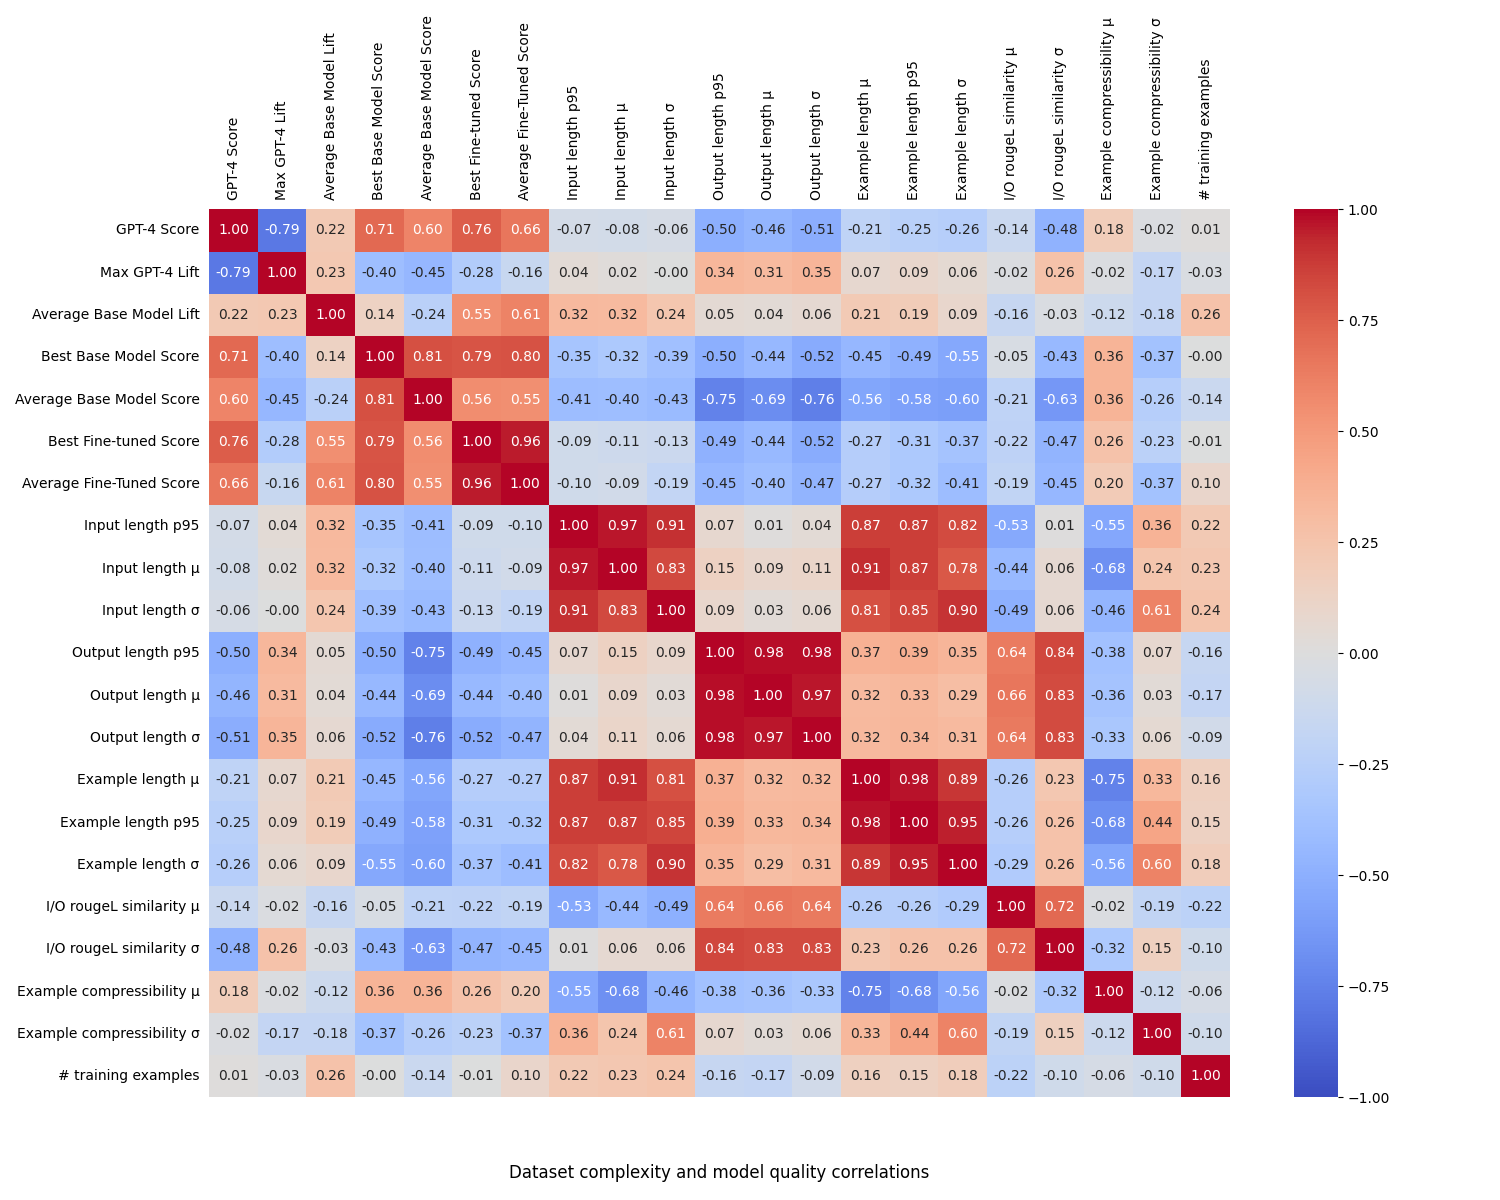
\includegraphics[width=\textwidth]{figures/task_correlation_matrix.png}
    \caption{Correlations between dataset complexity and model quality correlations for 310 LLMs across 31 tasks, before and after LoRA-based fine-tuning.}
\end{figure}

\subsubsection{Predicting fine-tuning quality and quality lift given task complexity heuristics}

We train linear regression models to predict the quality lift achievable through adapter-based fine-tuning, using z-score normalized dataset complexity heuristics (described in Table \ref{table:datasetcomplexityheuristics}) as predictors. Results are summarized in Table \ref{table:liftpredictionresults}, where we find that linear models yield root mean squared errors (RMSE) of 0.166 to 0.092, depending on the model quality metric in question.

Incorporating the score of the average base model without fine tuning as an additional feature improves prediction accuracy for all model quality metrics (+0.004 to +0.069). This demonstrates some predictive power in knowing base model performance for anticipating potential gains from fine-tuning. RMSE errors are rather low, suggesting that upfront heuristics-based measurements of dataset complexity can be reasonable indicators of positive fine-tuning impact.

\begin{table*}[ht]
\centering
\scalebox{0.8}{
\begin{tabular}{ccc}
\textbf{Model Quality Metric} & \textbf{\begin{tabular}[c]{@{}c@{}}With average base model score \\ as a feature \\ (RMSE)\end{tabular}} & \textbf{\begin{tabular}[c]{@{}c@{}}With average base model score\\ as a feature\\ (RMSE)\end{tabular}} \\
\midrule
GPT-4 Score                   & 0.140                                                                                                    & 0.121                                                                                                  \\
Max GPT-4 Lift                & 0.092                                                                                                    & 0.085                                                                                                  \\
Average Base Model Score      & 0.099                                                                                                    & N/A (0.000)                                                                                            \\
Best Base Model Score         & 0.166                                                                                                    & 0.097                                                                                                  \\
Average Base Model Lift       & 0.099                                                                                                    & 0.095                                                                                                  \\
Average Fine-Tuned Score      & 0.119                                                                                                    & 0.095                                                                                                  \\
Best Fine-tuned Score         & 0.097                                                                                                    & 0.091                                                                                                 
\end{tabular}
}

\caption{The performance of linear regression models predicting model quality heuristics before and after fine-tuning, given z-score normalized dataset complexity heuristics, with and without a representative base model score.}
\label{table:liftpredictionresults}

\end{table*}